\chapter{Crittografia Simmetrica}

\begin{figure}[h]
    \centering
    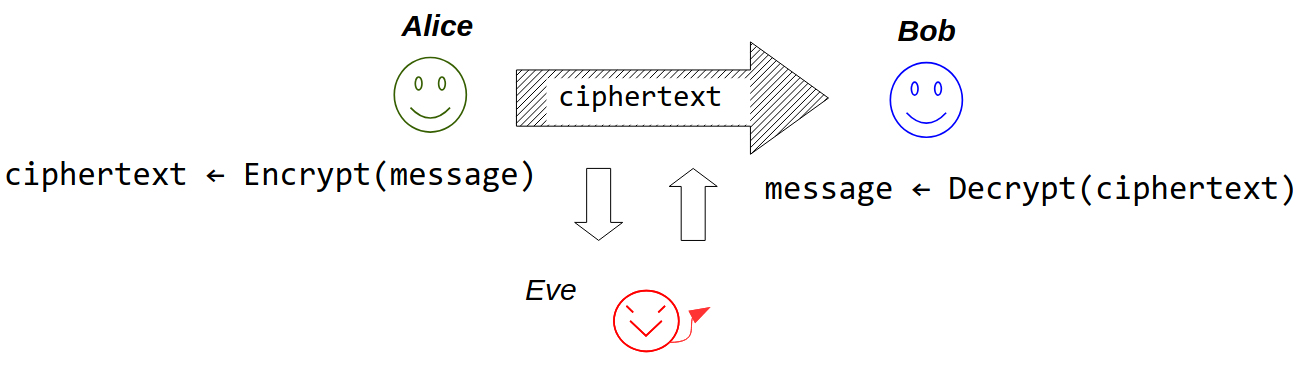
\includegraphics[width=\textwidth]{img/crypto_symm_1.png}
\end{figure}

Le garanzie di sicurezze che si cercano di mantenere sono:
\begin{itemize}[nosep]
    \item \textbf{confidenzialità}: Eve non può accedere a nessuna della informazioni sul messaggio.
    \item \textbf{autenticazione}: Bob può verificare se il messaggio non è stato inviato da Alice, viene anche chiamata \textbf{\textit{data orgin authenticity}} nel contesto della comunicazioni e implica anche la protezione contro modifiche illegittime (\textbf{integrità}).
\end{itemize}

\begin{flushleft}
    La sicurezza non esiste in natura è quindi necessario idearla e modellarla, questa prima parte prende il nome di \textit{Definitional Activity}. È comunque importante ricordare che le \textbf{definizioni} possono essere \textbf{errate} principalmente per errori nella modellazione o nello sviluppo software, ma anche perché non si è stato in grado di modellare quello che era invece richiesto. Un altro errore che si può essere portati a fare è quello di utilizzare in maniera errata certe definizioni ad esempio al di fuori del contesto per cui era stata definita. \newline
    \textbf{\textit{Definitional Activity}}: permette di descrivere che cosa l'avversario può \textbf{fare} e cosa può \textbf{vedere}. Esistono molteplici modi per definire la sicurezza in maniera più formale, uno tra questi è la \textbf{\textit{simulation-based security}} dove viene definita una funzione ideale che soddisfa la definizione di security e poi dimostrare che la funzione costruita si comporti come quella ideale.
\end{flushleft}

\begin{figure}[h]
    \centering
    \begin{large}
        \textbf{\textit{First Adversary Model}} \\
    \end{large}
    Quindi modelliamo e identifichiamo le casistiche e tipologie di un attaccante. \\

    \begin{minipage}[t]{0.50\textwidth}
        \centering
        \begin{boxA}
            \textcolor{red}{\textbf{\textit{Attack Model: Passive Eavesdropper (EAV)}}} \\
            Ha capacità di lettura dei soli \textit{ciphertext} e non è capace di \textbf{scegliere nulla}
        \end{boxA}
    \end{minipage}
    \begin{minipage}[t]{0.45\textwidth}
        \centering
        \begin{boxA}
            \textcolor{red}{\textbf{\textit{Security Goal: Indistinguishably}}} \\
            L'avversario non può distinguere il \textit{ciphertext} da sequenza di caratteri random.
        \end{boxA}
    \end{minipage}
\end{figure}

\begin{flushleft}
    Modellando in questo modo il nostro avversario è possibile osservare che non viene descritto nulla sul nascondere la lunghezza del \textit{plaintext}, infatti per questa prima modellazione l'avversario può vedere la lunghezza del \textit{plaintext}. \\
    \textbf{Nota}: la crittografia non ha come obiettivo quello di nascondere la lunghezza del testo in chiaro, nel caso in cui questa informazione fosse confidenziale, è necessario proteggerla a livello applicativo.
\end{flushleft}

\begin{flushleft}
    Le capacità di un avversario vengono espresse e descritte tramite degli algoritmi chiamati \textbf{esperimenti}, che vengono eseguiti da un'entità chiamata \textbf{\textit{challenger}} (che per semplicità andiamo ad identificare nell'attore onesto). \\
    Come prima andiamo ad analizzare \textbf{\textit{IND-EAV}}, il \textit{challenger} va a scegliere un messaggio \textbf{m} che viene scelto con la stessa probabilità tra:
    \begin{itemize}[nosep]
        \item dati random: $m \leftarrow \{0, 1\}^n$
        \item un messaggio generato attraverso la cifrazione $m = \text{Encryption}(p)$, dove \textbf{p} può essere scelto nello stesso modo di prima $p \leftarrow \{0, 1\}^n$
    \end{itemize}
    All'avversario viene fornito \textbf{m} e deve scegliere se è un messaggio randomico o se è l'output dell'\textit{encryption}, l'avversario vince l'esperimento se la sua decisione è corretta.
\end{flushleft}

\begin{flushleft}
    \textcolor{red}{\textbf{\textit{IND-EAV: Perfect \& Computational Indistinguishably}}} \\
    Andremo a discutere due tipologie di sicurezza:
    \begin{enumerate}[nosep]
        \item \textbf{\textit{perfect}}: la probabilità dell'avversario di vincere l'esperimento è del \textbf{50\%}, viene anche chiamata \textbf{\textit{Unconditional Security}} o \textbf{\textit{Informatition Theoretic Security}}.
        \item \textbf{\textit{computational}}: la probabilità dell'avversario di vincere l'esperimento è \textbf{50\%} più una \textbf{quantità trascurabile}.
    \end{enumerate}
    Qualunque tipologia di schema \textbf{praticabile} garantisce \textbf{sicurezza computazionale}, e se capace di essere sicuro contro un'\textbf{esperimento IND-EAV} viene detto \textbf{\textit{IND-EAV secure}}.
\end{flushleft}

\section{Sicurezza Incondizionata \& One-Time Pad}
\textcolor{red}{\textbf{XOR}}: gli schemi di crittografia moderni sono progettati per \textbf{dati binari}. L'operazione base per la crittografia simmetrica è lo \textbf{XOR}.

\begin{center}
    \begin{minipage}[c]{0.3\textwidth}
        \centering
        $c = m \oplus k$
    \end{minipage}
    \begin{minipage}[c]{0.3\textwidth}
        \centering
        \begin{tabular}{|c|c|c|}
            \hline
            \textbf{m} & \textbf{k} & \textbf{c} \\ \hline
            0 & 0 & 0 \\ \hline
            0 & 1 & 1 \\ \hline
            1 & 0 & 1 \\ \hline
            1 & 1 & 0 \\ \hline
        \end{tabular}
    \end{minipage}
    \begin{minipage}[c]{0.3\textwidth}
        \centering
        \textbf{Nota}: lo \textbf{XOR} può essere anche modellato come la somma bit per bit modulo 2: $c_i = (m_i \oplus k_i) \; \text{mod} \; 2$
    \end{minipage}
\end{center}

\begin{flushleft}
    Lo XOR viene scelto perché dato un certo \textbf{m}, se \textbf{k} viene scelta in maniera randomica la probabilità di \textbf{c} di essere \textbf{0} o \textbf{1} è \textbf{p = 0.5}. \\
    In questo modo sapere \textbf{c} non da informazioni su \textbf{m} e quindi \textbf{c} è indistinguibile da una successioni di bit random: $\{0, 1\}^n$
\end{flushleft}

\begin{flushleft}
    \textcolor{red}{\textbf{\textit{One-Time Pad - Vernam's Cipher}}}: è un algoritmo di crittografia che esegue un XOR bit a bit tra il testo in chiaro e la chiave, le due lunghezze devono essere uguali e la chiave devere essere random. $c_i = m_i \oplus k_i \; \forall i \in \{0, ..., n\}$ dove $n$ è la lunghezza del testo in chiaro. \\
    Per la decifrazione bisogna utilizzare la stessa chiave: $m = c \oplus k = (m \oplus k) \oplus k = m \oplus (k \oplus k) = m$. \\
    Anche se \textbf{OTP} è \textbf{incondizionatamente sicuro} non è praticabile realmente in quanto la generazione della chiave per testo arbitrario è computazionalmente onerosa ed è un algoritmo completamente \textbf{malleabile}. Gli schemi di crittografia oggi usati sono \textbf{computazionalmente sicuri}.
\end{flushleft}

\begin{flushleft}
    \textcolor{red}{\textbf{Nota sulla randomicità in crittografia}}: la randomicità in crittografia è differente da quella ``statistica'', ovvero una \textbf{distribuzione uniforme di 0 e 1} (che è necessaria ma non sufficiente), ma deve essere \textbf{\textit{unpredictable}}, in modo tale che anche osservando una sequenza, più o meno lunga di bit, non sia possibile predirre il bit successivo.
\end{flushleft}

\section{Sicurezza Computazionale: Security Level e Key Sizes}
Gli schemi crittografici moderni hanno come parte dei requisiti i \textbf{\textit{Kerckhoffs principle}} e necessitano uno \textbf{spazio delle chiavi largo} abbastanza per prevenire attacchi di ricerca esaustiva. Inoltre lo schema deve essere progettato in modo che si possa prevenire crittanalisi sul crittogramma, quindi nessuna informazione deve essere ottenuta dal crittogramma indipendentemente dal tipo di dato e deve essere sicura contro l'esperimento IND-EAV. 

Le condizioni necessarie avere degli schemi computazionalmente sicuri sono:
\begin{itemize}[nosep]
    \item gli schemi utilizzati devono essere computazionalmente sicuri.
    \item definiamo $F_k$ come una \textbf{PRF - \textit{Pseudo-Random Function}} con una chiave fissa \textbf{k} scelta randomicamente.
    \begin{itemize}[nosep]
        \item la \textbf{chiave} deve essere ``\textbf{corta}'' (ma lunga abbastanza per resistere ad attacchi a forza bruta).
        \item deve essere capace di cifrare grandi moli di dati.
        \item data la \textbf{chiave} le funzioni di \textbf{\textit{encryption}} e \textbf{\textit{decryption}} devono essere \textbf{efficenti}.
        \item senza la \textbf{chiave} la probabilità di rompere lo schema crittografico deve essere \textbf{trascurabile}.
    \end{itemize}
\end{itemize}

\begin{flushleft}
    È necessario tradurre in termini algoritmici \textbf{efficenti} e \textbf{trascurabile}. Alice e Bob che usano la funzione di \textit{encryption} e \textit{decryption} con la chiave devono essere capaci di eseguire gli algoritmi con costo \textit{efficient}, quindi il \textbf{costo computazionale} e \textbf{di memorizzazione} sono \textbf{polinomiali} sui parametri di sicurezza. Eve, che non conosce la chiave deve operare in maniera attraverso algoritmi \textbf{inefficienti}. \\
    $\rightarrow$ se il costo dell'attacco diverge da quello degli attori legittimi, è possibile scegliere i parametri di sicurezza appropriati in modo tale che la probabilità di completare correttamente l'algoritmo si molto piccola: \textbf{trascurabile}. 
\end{flushleft}

\begin{flushleft}
    Se fissiamo come probabilità di successo per definire un attacco a \textit{brute force} \textbf{inefficiente} $10^{-6}$, identifichiamo il valore di \textbf{N} per funzioni che hanno costo computazionale diverso, per quali valori di \textbf{n > N} le probabilità di sucesso sono inferiori?

    \begin{center}
        \begin{tabular}{lllll}
            \textbf{Costo di Esecuzione} && \textbf{Probabilità di Successo} && \textbf{\textit{Threshold}, b = 2} \\
            $\mathbf{O}(b^n)$ & $\rightarrow$ & $\mathbf{O}(b^{-n})$ & $\rightarrow$ & \textbf{N = 20} \\
            $\mathbf{O}(b^{\sqrt{n}})$ & $\rightarrow$ & $\mathbf{O}(b^{- \sqrt{n}})$ & $\rightarrow$ & \textbf{N = 400} \\
            $\mathbf{O}(b^{\log n})$ & $\rightarrow$ & $\mathbf{O}(b^{- \log n})$ & $\rightarrow$ & \textbf{N = 32}
        \end{tabular}
    \end{center}
    La conoscenza del costo dell'attacco più noto determina il valore del parametro di sicurezza, tra gli altri, la \textbf{dimensione della chiave}, identificato dal valore \textbf{N}.

    {\centering
        $\exists N \; | \; f(n) < \frac{1}{p(n)}, \; \forall n < N$
    \par}
\end{flushleft}

\begin{boxA}
    \textcolor{orange}{\textbf{Esempio}} \\
    Definiamo il costo di cifrazione $c_{enc}(n) = n$ mentre il costo dell'attacco $c_{attack} = n^2$ dove $n$ è la lunghezza della chiave. \\
    Negli anni 2000 l'\textit{encryption} utilizzava una chiave a 64bit e impiegava 1ms, mentre l'attacco a forza bruta, impiegava 2 anni. Dopo 10 anni, nel 2010, con la stessa chiave la cifrazione impiegava 0.1ms e il suo brute force 2 mesi. \\ \newline
    Aumentando la lunghezza della chiave, raddoppiandola, la fase di cifrazione impiegava 0.2ms, mentre quella di \textit{brute force} passava da $2^{64}$ a $2^{128} \simeq 10^{20}$ mesi.
\end{boxA}

\begin{flushleft}
    Grazie a nuove scoperte vengono trovati algoritmi che \textbf{indeboliscono} o \textbf{compromettono} il cifrario. Ad esempio alcuni schemi vengono pubblicamente violati pochi anni dopo la loro scoperta come gli schemi crittografici della famiglia \textit{rc} o \textit{sha1}. È anche possibile che schemi standard vengano indeboliti attraverso \textit{backdoor}, parametri deboli o ``particolari'' e implementazioni deboli.
\end{flushleft}

\begin{flushleft}
    \textcolor{red}{\textbf{\textit{Efficient function}}} $\rightarrow$ \textbf{\textit{polynomial}} \\
    Il costo (computazionale e memorizzativo) sono polinomiali rispetto ad un certo parametro di sicurezza $n$, algoritmi di \textit{encryption} costano al massimo: 
    
    {\centering
        $p(n) := a \cdot n^x$
    \par}

    \textcolor{red}{\textbf{\textit{Negligible function}}} $\rightarrow$ \textbf{\textit{smaller that any inverse polynomial}} \\
    Esiste un valore di \textbf{N} tale che la funzione sia minore di qualsialsi funzione polinomiale:

    {\centering
        $\exists N \; \text{t.c.} \; f(n) < \frac{1}{p(n)}, \; \forall \; n < N$
    \par}
\end{flushleft}

\begin{flushleft}
    \textcolor{red}{\textbf{\textit{PseudoRandom functions}}} \\
    Definiamo una \textbf{funzione ideale} che soddisfa computazionalmente l'esperimento di sicurezza IND-EAV, nel caso di crittografia a chiave privata, questo tipo di funzione si chiama \textbf{\textit{(keyed) family of PseudoRandom Function (PRF)}}.

    {\centering
        $\mathbf{F} \; : \; \mathbf{K} \times \mathbf{P} \mapsto \mathbf{C}$
    \par}

    Dove:
    \begin{itemize}[nosep]
        \item \textbf{K} è uniformemente scelto da $\{0, 1\}^{Lk(n)}$
        \item \textbf{P} è il \textit{plaintext} scelto arbitrariamente da $\{0,1\}^{Lp(n)}$
        \item \textbf{C} soddisfa computazionalmente \textbf{IND-EAV}, dove la ``quantità trascurabile'' è espressa dalla funzione \textbf{negl(n)} 
    \end{itemize}

    Uno schema di crittografia deve essere \textbf{funzionale}. Definiamo \textbf{F} come la \textbf{PRF} allora \textbf{F} si definirà computazionalmente sicura se:
    \begin{itemize}[nosep]
        \item lo spazio della chiavi è ``\textbf{piccolo}'', ma grande a sufficienza per resistere ad attacchi basati su ricerca esaustiva. Quindi $Lk(n)$ \textbf{deve} essere una funzione efficiente.
        \item ha la capacità di generare in output grande quantità di dati \textbf{\textit{pseudorandom}} (è sicuro per IND-EAV).
        \item il costo di computazione di \textbf{F} è \textbf{efficiente}.
        \item senza la chiave, la probabilità di rompere lo schema crittografico è \textbf{trascurabile}, il costo di calcolare $\mathbf{F}^{-1}$ è \textbf{inefficiente}.
    \end{itemize}
\end{flushleft}

\begin{flushleft}
    \textcolor{red}{\textbf{\textit{Concrete parameters for acceptable security guarantees}}} \\
    Gli schemi di crittografia (simmetrica) moderni vengono considerati computazionalmente sicuri, tali schema possono essere violati se si dispone di abbastanza tempo e abbastanza risorse. \\
    Il \textbf{\textit{Security Level}} dello schema è la media del numero di operazioni necessarie per rompere lo schema: gli standard stabiliscono dei valori tali che la quantità di tempo e risorse necessaria per calcolare tale quantità di operazioni è \textit{unfeasible}.
    \begin{itemize}[nosep]
        \item 80-bit di sicurezza $\rightarrow \; 2^{80}$ operazioni in media per rompere lo schema (insicuro dal 2010).
        \item 112-bit di sicurezza $\rightarrow \; 2^{112}$ operazioni in media per rompere lo schema (insicuro dal 2030).
        \item 128-bit di sicurezza $\rightarrow \; 2^{128}$ operazioni in media per rompere lo schema (stimata la sicurezza per ogni scenario successivo).
    \end{itemize}

    Nei moderni \textbf{schemi di crittografia simmetrica}, la \textbf{lunghezza della chiave} definisce il \textbf{livello di sicurezza}, in quanto l'attacco \textit{best-known} è basato sull'indovinare il segreto. A differenza, negli \textbf{schemi di crittografia asimmetrica} dove invece è presente solo una correlazione, in quanto dipende dagli attacchi noti alla matematica sottostante. \\

    Software e librerie \textbf{dovrebbero} implementare configurazioni \textbf{sicure} di \textbf{default} e aggiornate se necessarie
\end{flushleft}

\begin{flushleft}
    \textcolor{red}{\textbf{\textit{Asymmetric Cryptography \& Quantum Computers (PQC)}}} \\
    Si stima che gli attuali standard di crittografia asimmetrica saranno efficacemente violati dai computer quantistici nei prossimi decenni. Nell'ultimo decennio, sono stati ipotizzati e analizzati a fondo nuovi problemi cosiddetti ``\textbf{\textit{post-quantum hard problems}}'', ovvero che non possono essere risolti in modo efficiente nemmeno con un computer quantistico.
\end{flushleft}

\section{Stream Cipher}